\documentclass[a4paper]{article}

\usepackage[utf8]{inputenc}
\usepackage[portuguese]{babel}	
\usepackage{graphicx}
\graphicspath{ {Imagens/} }

\title{Trabalho Prático 3 de Processamento de Linguagens}
\author{André Vieira (A78322) \and Eduardo Rocha (A77048) \and Ricardo Neves (A78764)}
\date{\today}

\begin{document}

\maketitle

\begin{abstract}
  Este documento apresenta o relatório do terceiro projeto de Processamento de Linguagens, 
  de Mestrado Integrado em Engenharia Informática da Universidade do Minho.
  Aqui, será realizada a descrição de todo o trabalho realizado pelo grupo, que
  consistiu em escolher uma gramatica e desenvolver um reconhecador lexico.

\end{abstract}

\tableofcontents

\vspace{150px}
\section{Introdução}
\label{sec:intro}

Este trabalho prático foi realizado no ambito da Unidade Curricular de Processamento de Linguagens.
Aqui, iremos dicutir toda a estratégia e linha de pensamento que o grupo tomou, de modo a cumprir os requisitos pedidos.

Uma vez que o menor número mecanográfico é igual a 77048, e ao dividir este mesmo número por 8, constatamos que o resto desta operação é igual a 0. Assim, 0+1=1, o que corresponde ao número do exercicio a realizar.

Deste modo, o grupo constatou que o enunciado atribuido foi o 3.1 - Rede Semântica do Museu da Emigração.
Este trabalho engloba, em geral, 2 exercícios distintos, que iremos mencionar mais à frente, em pormenor.
O objetivo máximo do grupo em relação a este trabalho foi o de realizar o exercício com a maior eficiência, ganhando, assim, experiência e conhecimento em relação ao FLEX e a reconhecedores léxicos, que irá ser importante no seguimento desta Unidade Curricular. 
Com o fecho da introdução deste relatório, é adequado mencionar a estrutura do mesmo. Este relatório contém o resumo do trabalho que foi realizado durante o período dado para tal, a descrição e a implementação do exercício que do trabalho prático (incluíndo a linha de pensamento seguida pelo grupo, bem como imagens que ajudam à interpretação), e no final, uma pequena conclusão que reflete o trabalho realizado.

\vspace{300px}
\section{Resumo}
\label{sec:resumo}

Neste terceiro exercício, pretende-se descrever parte da rede semantica que suporta o Museu da Emigração, das Comunidades e da Luso-Descendencia. Deste modo, gera-se um grafo (usando GraphVIZ ou DOT) que permita uma navegação sobre esta base de dados. Esta rede conta com 3 nodos, ou vértices: o emigrante (caracterizado pelo nome, idade, concelho, destino e código), a obra (podendo se tratar de um palácio, fábrica, hospital, etc.) ou um evento (por exemplo, baile, sarau, etc.). A isto, alia-se os nodos entre os vértices: fez (que liga o emigrante a uma obra), e participou (que liga um emigrante a um evento). 

\vspace{500px}
\section{Rede}
\label{sec:gawk}

De modo a ir testando a implementação do grupo, criamos uma pequena rede com exemplos retirados do site indicado pelos docentes.
Assim, esta é a rede semantica utilizada, e que será descrita na forma de um grafo:

\begin{center}
	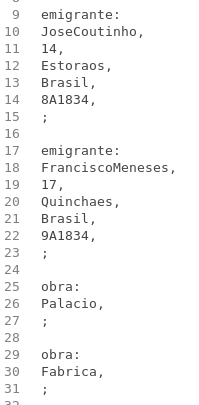
\includegraphics[scale=0.85]{rede}
	\begin{figure}[!ht]
	\caption{Rede semântica de teste}
	\end{figure}
\end{center}

Em cima, podemos verificar que o tipo do nodo é seguido por dois pontos ':' e, só depois, todos os dados relativos a esse emigrante, por exemplo.
No fim de um dado, deve-se acabar com uma vírgula.
Para fechar este nodo, utiliza-se o ponto e virgula. Aqui, o programa irá saber que este nodo terminou, e irá procurar por mais.
Esta foi a gramática escolhida consensualmente pelo grupo, depois de vários testes a outras gramáticas.

\vspace{100px}
\section{YACC}
\label{sec:yacc}

Uma vez concebida a gramática do projeto, e todos os dados inseridos na mesma, é altura de ler esse ficheiro e armazenar em estruturas de dados, essas mesmas informações.
O grupo decidiu dividir todas as informações nos seus Arrays de Strings apropriados. Por exemplo, todos os nomes de todos os emigrantes estão guardados no Array Nome. Com isto, é muito mais fácil, posteriormente, construir o grafo.
Para isto, foi implementado um ficheiro YACC, onde dividimos a grmática em vários blocos. Cada bloco criado é responsável pela leitura e junção de todas as informações que são recebidas pelo ficheiro onde se encontram todos os dados dos emigrantes, obras e eventos.

\begin{center}
	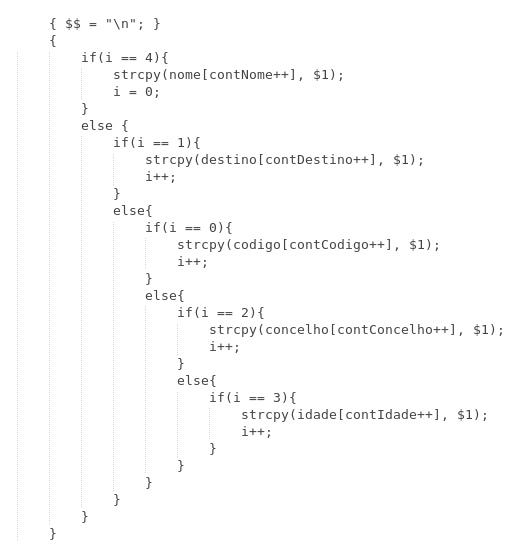
\includegraphics[scale=0.72]{yacc}
	\begin{figure}[!ht]
	\caption{Excerto do ficheiro YACC}
	\end{figure}
\end{center}

Em cima, apresentamos um excerto do YACC criado para a leitura da gramática desenvolvida. Colocar aqui todo o ficheiro YACC não é o mais aconselhado, devido á dimensão do mesmo.
No entanto, neste excerto de código, podemos ver a parte responsável por ler e armazenar os dados dos vários emigrantes. Assim, usamos várias variáveis auxiliares e, dependendo da ordem em que os dados apareciam, eram guardados no Array destinado.

\vspace{500px}
\section{FLEX}
\label{sec:gawk}

O código YACC acima referido tem de ser auxiliado por uma implementação FLEX que ajuda no parse dos dados.

\begin{center}
	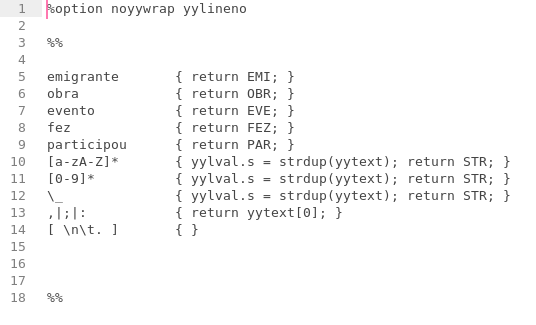
\includegraphics[scale=0.7]{flex}
	\begin{figure}[!ht]
	\caption{Ficheiro FLEX}
	\end{figure}
\end{center}

Como podemos ver, utilizamos uma série de expressões regulares para dividir os dados.
Por exemplo, sempre que é encontrada a palavra emigrante, o FLEX dá a conhecer ao YACC que irá ler, de seguida, os dados de um emigrante. Isto é igual para o resto das entidades.
Foram também criadas expressões regulares para a leitura de palavras, números e underscores. Tudo o resto será ignorado pelo  programa.

\vspace{200px}
\section{Resultado Final}
\label{sec:resfinal1}

Para um teste mais rápido deste exercício, o grupo criou a seguinte Makefile:

\begin{center}
	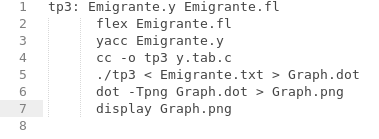
\includegraphics{makefile}
	\begin{figure}[!ht]
	\caption{Makefile do exercício}
	\end{figure}
\end{center}

Ao correr esta Makefile, será aberta uma imagem do grafo concebido ao longo do exercício.

\begin{center}
	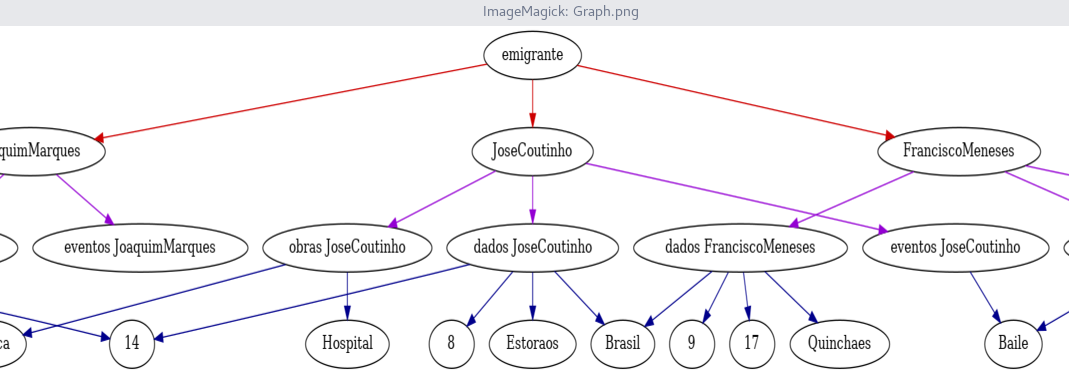
\includegraphics[scale=0.35]{grafo}
	\begin{figure}[!ht]
	\caption{Grafo resultante}
	\end{figure}
\end{center}

Como se pode observar, no topo, estão presentes todos os emigrantes da base de dados.
Cada emigrante desenvolve-se em 3 grupos: dados, obras e eventos a que o emigrante foi.
Em baixo de cada nodo, é apresentada a informação relativa.

Depois de algumas pesquisas, o grupo não conseguiu implementar um grafo interativo onde, clicando em cada nodo, iria ser possível observar toda a informação contida no mesmo. Temos a noção que é um ponto onde o grupo falhou e que, com mais tempo e uma pesquisa mais aprofundada, este requisito seria completamente coberto.

\vspace{100px}
\section{Conclusões}
\label{sec:conclusao}

Com este trabalho prático, adquirimos e, maioritariamente, aprofundamos os nossos conhecimentos acerca do gerador FLEX e do YACC. Com isto, constatamos toda a utilidade que estas ferramentas, juntas, nos podem oferecer, sendo que agora, com estes exercícios, conseguimos dominar melhor as mesmas.
Em suma, estamos satisfeitos com o trabalho realizado até então, sendo que o grupo se sente preparado para, após este desenvolvimento dos conhecimentos em FLEX e YACC que irão ser importantes no futuro.

\end{document}